\documentclass{sig-alternate}
%\documentclass[10pt]{sigplanconf}

\usepackage{booktabs}
\usepackage{colortbl}
\usepackage{tabularx}
\usepackage{multirow}
\usepackage{color}
\usepackage{xspace}
\usepackage{hyperref}    % Creates hyperlinks from ref/cite 
\hypersetup{pdfstartview=FitH}
\usepackage{graphicx}    % For importing graphics
\usepackage{url}         %
\usepackage{verbatim}
\usepackage{amssymb}
\usepackage{amsmath}
\relpenalty=9999
\binoppenalty=9999

\newcommand{\2}{\;\;}
\newcommand{\5}{\;\;\;\;\;}
\newcommand{\brk}{\textbf{\small{$^\wedge$}}}
\newcommand{\CEU}{\textsc{C\'{e}u}}
\newcommand{\nesc}{\emph{nesC}}
\newcommand{\code}[1] {{\small{\texttt{#1}}}}
\newcommand{\Code}[1] {\texttt{#1}}

\begin{document}

%\conferenceinfo{Onward! '12}{date, City.}
%\copyrightyear{2012}
%\copyrightdata{[to be supplied]}

\title{Safe and High-level Programming for Embedded Systems}

\begin{comment}
\author{Francisco Sant'Anna, Noemi Rodriguez, Roberto Ierusalimschy\\
        Departamento de Inform\'atica --- PUC-Rio, Brasil\\
        \{fsantanna,noemi,roberto\}@inf.puc-rio.br}

\authorinfo{Name1}
           {Affiliation1}
           {Email1}
\authorinfo{Name2\and Name3}
           {Affiliation2/3}
           {Email2/3}

\maketitle

\begin{abstract}
In this work, we support the adoption of safety and high-level capabilities 
found in synchronous languages for the design of embedded systems.
The synchronous programming model provides deterministic concurrency, offering 
a reliable alternative to $C$-based systems.

Using two complete demo applications, we describe typical patterns in embedded 
systems and discuss how language support leads to straightforward 
implementations with extra safety warranties.

We use the programming language \CEU{} for implementing the examples.
\CEU{} supports shared-memory concurrency, but its synchronous nature enables a 
compile time analysis that can enforce deterministic and memory-safe programs.
With a good balance between low-level and high-level functionality, \CEU{} fits 
the constrained requirements of embedded systems.
\end{abstract}

%\category{D.3}{Programming Languages}{General}
\category{D.3.3}{Programming Languages}{Language Constructs and Features}

%\terms{Design, Languages}
\terms{Experimentation, Reliability, Verification}

\keywords{Synchronous, Determinism, Safety, Embedded Systems}

\section{Introduction}
\label{sec:intro}

Embedded systems differ from general-purpose systems and are designed to 
perform specific and dedicated tasks within large systems.
Usually, they are constrained in memory and processing, and have low tolerance 
to faults.

Software for embedded systems is usually developed in $C$, given its 
flexibility and low-level capabilities, which are important requirements in the 
context of embedded systems.
The addition of a real-time operating system may extend it with cooperative 
and/or preemptive multithreading.
However, concurrency in $C$ requires an arduous and error-prone exercise 
related to the life cycle and synchronization of activities.
Furthermore, these models lack safety warranties, given that they are 
susceptible to unbounded execution~\cite{wsn.sol} (i.e. infinite loops), and/or 
nondeterminism~\cite{sync_async.threadsproblems}.

An alternative for designing embedded systems is the synchronous programming 
model, in which time is divided in discrete instants that compute reactions to 
the environment atomically.
A primeval goal for synchronous languages is to ensure the correctness of 
programs through static verification.~\cite{rp.twelve}

%\CEU{}~\cite{ceu.tr} is an example of a high-level synchronous language that 
\CEU{}\footnote{\url{http://www.ceu-lang.org}} is a high-level synchronous 
language that supports lock-free shared-memory concurrency, but preserves 
low-level functionality via inlined $C$.
To conform with safety requirements, \CEU{} relies on a compile-time analysis 
that detects concurrent access to variables and $C$ calls.

In this work, we promote the use of \CEU{} for embedded development through an 
empirical approach.
We depict two complete applications in different domains in order to expose the 
language features related to issues such as deterministic concurrency, error 
recovery, and safe access to shared variables.
We demonstrate how high-level language support can assist low-level 
manipulation to achieve safer code.

Current works (discussed in Section~\ref{sec:related}) either focus on 
justifying language features through small code snippets, or by performing a 
quantitative analysis on a reasonable set of programs, which are never 
discussed in detail.
We believe that a careful explanation of more complete applications can help 
the reader to grasp the synchronous programming mindset.
%TODO: and why it can be beneficial for embedded systems.

We briefly introduce \CEU{} in Section~\ref{sec:ceu}, focusing on the provided 
high-level compositions and safety warranties.
In Section~\ref{sec:demos}, we present the two embedded demo applications in 
detail.
In Section~\ref{sec:related}, we compare existing high-level alternatives for 
embedded programming, arguing that \CEU{} provides unique features not present 
in other systems.
In Section~\ref{sec:conclusion}, we make final remarks and conclude the paper.

\section{The Language C\'eu}
\label{sec:ceu}

\CEU{} is a reactive language that supports multiple lines of execution---known 
as \emph{trails}---that continuously react to external input events broadcast 
by the environment.
The introductory example that follows executes two trails in parallel through 
the \code{par} statement to wait for different events at the same time:

{\small
\begin{verbatim}
   1:  input int Restart;   // declares an external event
   2:  int v = 0;
   3:  par do
   4:     loop do           // 1st trail
   5:        await 1s;
   6:        v = v + 1;
   7:        _printf("v = %d\n", v);
   8:     end
   9:  with
  10:     loop do           // 2nd trail
  11:        v = await Restart;
  12:     end
  13:  end
\end{verbatim}
}

The declared input event \code{Restart} triggers an integer value when it 
occurs (line 1).
The loop in the first trail (lines 4-8) continuously waits for 1 second, 
increments variable \code{v}, and prints its current value.
The loop in the second trail (lines 10-12) resets \code{v} on every occurrence 
of \code{Restart}.

Symbols defined externally in $C$%
\footnote{Symbols for functions, types, globals, and constants available in the 
$C$ compiler for the target embedded platform.
}, such as \code{printf} in the example, must be prefixed with an underscore to 
be used in \CEU{} programs.

The synchronous execution model of \CEU{} states that only a single reaction to 
an external event can execute at a time, and also that reactions must run to 
completion. %~\cite{ceu.tr}.
In the example, after the program starts, both trails start and get suspended: 
the first awaits \code{1s}, while the second awaits event \code{Restart}.
After that, as both awaits are inside loops, the program may react multiple 
times to each of those events.
However, there is no possible race condition on variable \code{v} because 
reactions always execute atomically and are never interleaved, thus enabling 
lock-free concurrency in the language.

% first-class timers

The example illustrates the (simpler) reasoning about concurrency aspects under 
the synchronous execution model.
In contrast, in a model with nondeterministic scheduling, the occurrence of 
\code{Restart} could preempt the first trail during the increment (line 6) and 
set the value of \code{v} (line 11) before printing it (line 7), characterizing 
a race condition on variable \code{v}.

\subsection{High-level compositions}
\label{sec:ceu:high}

\begin{comment}
For instance, \emph{parallel compositions} help on the development of 
concurrent applications in which multiple peripherals are controlled at the 
same time.
\textbf{Composability (TODO: ?)}
\end{comment}

Programs in \CEU{} are structured with standard imperative primitives, such as 
sequences, loops, and assignments.
The extra support for parallelism allows programs to wait for multiple events 
at the same time.
Note that trails await events without loosing context information, such as 
locals and the program counter, what is a desired behavior in concurrent 
applications.~\cite{sync_async.cooperative}

The conjunction of parallelism with standard control-flow enable hierarchical 
compositions, in which self-contained blocks of code can be deployed 
independently.
To illustrate the expressiveness of compositions in \CEU{}, consider the two 
variations of the structure that follows:

{\small
\begin{verbatim}
    loop do                     loop do
        par/and do                  par/or do
            ...                         ...
        with                        with
            await 1s;                   await 1s;
        end                         end
    end                         end
\end{verbatim}
}

In the \code{par/and} loop variation, the code in the first trail (represented 
as \code{...}) is repeated every second at minimum, as the second trail must 
also terminate to rejoin the \code{par/and} primitive and restart the loop.

In the \code{par/or} loop variation, if the code does not terminate within a 
second, the second trail rejoins the composition (cancelling the first trail) 
and restarts the loop.

These structures represent, respectively, the \emph{sampling} and 
\emph{watchdog} patterns, which are common in embedded applications.

Note that the body of \textbf{\code{...}} may contain arbitrary code with 
nested compositions and awaits, but the described patterns will work as 
expected.
Even if the code share globals, the program as a whole is analysed at compile 
time in order to detect inconsistencies (to be discussed in 
Section~\ref{sec:ceu:safety}).

Structured programming with local scopes and parallel compositions is not a 
privilege of synchronous languages.
For instance, threads in $C$ have stacks to hold local variables, while 
processes in message-passing systems are easily composable with a single 
operator.
However, synchronous languages provide a more accurate control of the life 
cycle of concurrent activities.
For instance, the code snippet that follows specifies that code \code{<P>} 
should be aborted exactly when event \code{E} occurs, and then code \code{<Q>} 
should execute:

\begin{verbatim}
    par/or do
        <P>         // a self-contained composition
    with
        await E;    // the preempting event
    end
    <Q>             // subsequent composition
\end{verbatim}

The \code{par/or} statement is regarded as an \emph{orthogonal preemption 
primitive}~\cite{esterel.preemption}, because composition \code{<P>} does not 
know when and why it gets aborted by event \code{E}.

In a similar (hypothetical) construct for an asynchronous language, the 
occurrence of event \code{E} would not imply the immediate termination of 
\code{<P>}, which could continue to execute for an arbitrary amount of time.
Asynchronous formalisms assume time independence among processes and require 
explicit synchronization mechanisms.
Therefore, to achieve the desired specification, processes \code{<P>} and 
\code{<Q>} must be tweaked with synchronization commands, breaking the
orthogonality assumption.~\cite{esterel.preemption}

\subsection{Safety warranties}
\label{sec:ceu:safety}

Safety is an important aspect in embedded systems, given their reliability 
requirements.
Besides lock-free concurrency, \CEU{} ensures at compile time that reactions to 
events execute in bounded time and are deterministic.%~\cite{ceu.tr}

\textbf{Bounded execution}

Reactions to the environment should run in bounded time to guarantee that 
programs are responsive and can handle upcoming input events.
\CEU{} requires that each possible path in a loop body contains at least one 
\code{await} or \code{break} statement, thus ensuring that loops never run in 
unbounded time.

Consider the examples that follow:

{\small
\begin{verbatim}
    loop do                     loop do
        if v > 1000 then            if v > 1000 then
            break;                      break;
        end                         else
        v = v + 1;                      await 1s;
    end                             end
                                    v = v + 1;
                                end
\end{verbatim}
}

The first example is refused at compile time, because the \code{if} true branch 
may never execute, resulting in an infinite loop.
The second variation is accepted, because for every iteration, the loop either 
escapes or awaits.

Note that \CEU{} does not extend this analysis for $C$ function calls.
In this case, the responsibility to ensure bounded execution is left to the 
programmer.

\textbf{Deterministic execution}

\begin{figure}[t]
\centering
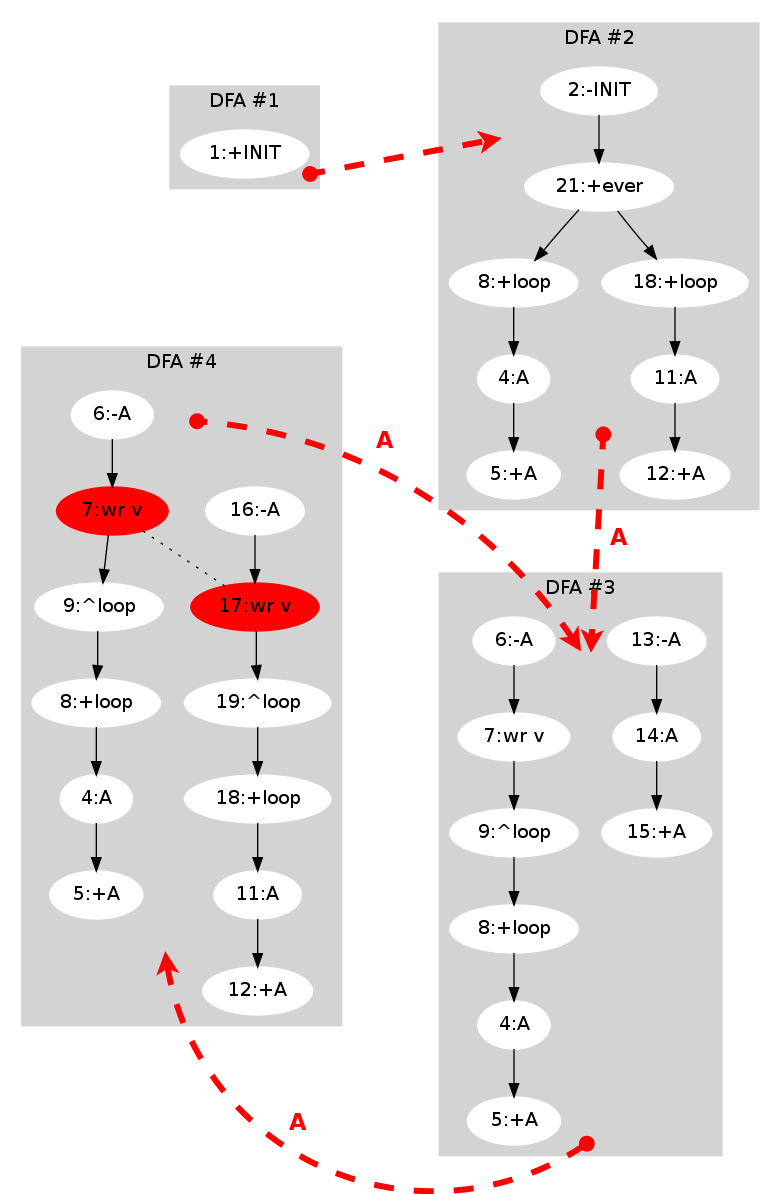
\includegraphics[scale=0.25]{dfa.png}
\caption{ DFA for the nondeterministic example.
\label{fig:dfa}
}
\end{figure}

Determinism is usually a desired safety property for programs, making 
concurrency predictable and easier to debug.
\CEU{} performs a compile-time analysis in order to detect nondeterminism in 
programs.
The static analysis relies on the synchronous execution model to generate a 
deterministic finite automata that covers all possible points a program can 
reach during runtime.

As an example, the DFA in Figure~\ref{fig:dfa} corresponds to the following 
program:

{\small
\begin{verbatim}
    input void A;
    int v;
    par do
        loop do
            await A;
            v = 1;
        end
    with
        loop do
            await A;
            await A;
            v = 2;
        end
    end
\end{verbatim}
}

After two occurrences of event $A$, variable \code{v} is accessed concurrently 
in the program, which is qualified as nondeterministic and is refused at 
compile time (note the outlined nodes in state \emph{DFA \#4}).
The same reasoning is done for concurrent $C$ calls with side effects, which 
are illustrated in Section~\ref{sec:demos:ring}.

\section{Demo applications}
\label{sec:demos}

In this section, we present two demos %
%\footnote{The complete source and a video demos for the applications can be 
%found at \url{http://www.ceu-lang.org/sac\_13/}.}
that explore the high-level and safety capabilities of \CEU{} described in the
previous section.
The applications are somewhat simple to fit the paper (70 and 170 lines), but 
still complete enough in order to expose the programming techniques promoted by 
the language.

The first demo targets Wireless Sensor Networks (WSNs), which are networks 
composed of a large number of tiny devices (known as ``motes'') capable of 
sensing the environment and communicating among them~\cite{wsn.survey}.
The second demo uses the Arduino open-source platform%
\footnote{\url{http://arduino.cc}},
a popular choice among hobbyists aiming to experiment with electronics in 
multidisciplinary projects.
Both platforms have low processing power and memory capacity, showing that 
\CEU{} is applicable to highly constrained platforms.

\subsection{WSN ring}
\label{sec:demos:ring}

In the first demo, we implement a fixed ring topology with $N$ motes placed 
side by side within their radio ranges.

All motes should follow the same behavior: receive a message with an integer 
counter, show it on the LEDs, wait for $1$ second, increment the counter, and 
forward it to the mote on its right.
%Note that using fixed topologies and running the same application in all motes 
%are common practices in the context of WSNs.

Because the topology constitutes a ring, the counter will be incremented 
forever while traversing the motes.
If a mote does not receive a message within $5$ seconds, it should blink the 
red LED every $500$ milliseconds until a new message is received.
%In a ring topology, communications traverse all motes, and the network goes 
%down with a failure in a single mote, making tests much easier.

The mote with \emph{id=0} is responsible for initiating the process at boot 
time.
Also, on perceiving the failure, it should wait for $10$ seconds before 
retrying the communication.

The communicating trail, which continuously receives and forwards the messages, 
is as follows:

{\small
\begin{verbatim}
     1:  loop do
     2:     _message_t* msg = await Radio_receive;
     3:     int* cnt = _Radio_getPayload(msg);
     4:     _Leds_set(*cnt);
     5:     await 1s;
     6:     *cnt = *cnt + 1;
     7:     _Radio_send((_NODE_ID+1)%N, msg);
     8:  end
\end{verbatim}
}

The code is an endless loop that first awaits a radio message (line 2), gets a 
pointer to its data buffer (line 3), shows the received counter on the LEDs 
(line 4), and then awaits $1$s (line 5) before incrementing the counter in the 
message (line 6) and forwarding it to the next mote (line 7).

The program uses several services provided by the underlying operating system 
(\cite{wsn.tos}), which are all non-blocking $C$ functions for LEDs and radio 
manipulation.

Because this code does not handle failures, it is straight to the point and 
easy to follow.
Actually, this is the final code for this task, as error handling is placed in 
a parallel trail.

Note that the program accesses the message buffer multiple times in reaction to 
events.
Because the \code{await} primitive provides sequential flow across reactions to 
events, every access to the buffer in the code is undoubtedly deterministic.
However, in typical event-driven systems~\cite{wsn.nesc}, the accesses would be 
split in multiple callbacks, requiring a thoughtful reasoning about concurrency 
issues.

To handle failures, we use a monitoring trail (lines 10-28) in parallel with 
the communicating trail:

{\small
\begin{verbatim}
     0:  par do
    (1-8):  // COMMUNICATING TRAIL (previous code)
     9:  with
    10:     loop do
    11:        par/or do
    12:           await 5s;
    13:           par do
    14:              loop do
    15:                 emit retry;
    16:                 await 10s;
    17:              end
    18:           with
    19:              _Leds_set(0);  // clear LEDs
    20:              loop do
    21:                 _Leds_led0Toggle();
    22:                 await 500ms;
    23:              end
    24:           end
    25:        with
    26:           await Radio_receive;
    27:        end
    28:     end
    29:  end
\end{verbatim}
}

Lines 12 to 24 describe the network-down behavior.
After $5$ seconds of inactivity is detected (line 12), two new activities run 
in parallel: one that retries communication every $10$ seconds by signaling the 
internal event \code{retry} (lines 14-17); and another that blinks the red LED 
every $500$ milliseconds (lines 19-23).

The trick to restore the normal behavior of the network is to await event 
\code{Radio\_receive} (line 26) in a \code{par/or} (line 11) with the 
network-down behavior to kill it whenever a new message is received.
By surrounding everything with a \code{loop} (line 10), we ensure that the 
error detection is continuous.
Note that this is exactly the watchdog pattern described in 
Section~\ref{sec:ceu:high}.

%Note that both the communicating trail and the monitoring trail waits for the 
%event \code{Radio\_receive} (lines 2 and 26, respectively), and both react 
%concurrently to it.
%The first is responsible for handling the message and forwarding it, while the 
%second just kills the network-down behavior (the blinking red LED).

Finally, we need to implement the initiating/retrying process that sends the 
first message from mote with \emph{id=0}.
Again, we place the code (lines 30-40) in parallel with other activities:

{\small
\begin{verbatim}
     0:  par do
    (1-8):   // COMMUNICATING TRAIL
     9:  with
    (10-28): // MONITORING TRAIL
    29:  with
    30:     if _NODE_ID == 0 then
    31:        loop do
    32:           _message_t msg;
    33:           int* cnt = _Radio_getPayload(&msg);
    34:           *cnt = 1;
    35:           _Radio_send(1, &msg)
    36:           await retry;
    37:        end
    38:     else
    39:        await Forever;
    40:     end
    41:  end
\end{verbatim}
}

We start by checking whether the mote has \emph{id=0} (line 30).
If this is not the case, we simply await forever on this trail (line 39)%
\footnote{\code{Forever} is a reserved keyword in \CEU, and represents an input 
event that never occurs.}.
Otherwise, the \code{loop} (lines 31-37) sends the first message as soon as the 
mote is turned on (line 35).
It then waits for a \code{retry} emit (line 36) to loop and resend the initial 
message.
Remind that event \code{retry} is emitted on network-down every $10$ seconds 
(line 15).

The static analysis of \CEU{} correctly complains about concurrent calls to 
\code{\_Radio\_send} (line 35) \emph{vs.} \code{\_Leds\_set} and 
\code{\_Leds\_led0Toggle} (lines 19,21), which all execute after the program 
detects 5 seconds of inactivity (line 12).
However, because these functions affect different devices (i.e. radio 
\emph{vs.} LEDs), they can be safely executed concurrently.
The following annotation (to be included in the program) states that these 
specific functions can be called concurrently with deterministic behavior, 
allowing the program to be compiled without errors:

{\small
\begin{verbatim}
    deterministic _Radio_send with
                  _Leds_set, _Leds_led0Toggle;
\end{verbatim}
}

\begin{comment}
As a final consideration, we can extend the idea of compositions by combining 
different \emph{applications} together.
In the context of WSNs, it is usually difficult to physically recover motes in 
a deployed network, and by combining multiple applications in a single image, 
we can switch their execution remotely via radio.
The following archetype illustrates this idea:

{\small
\begin{verbatim}
     1:   input int Switch;
     2:   int cur_app = 1;
     3:   loop do
     4:      par/or do
     5:         cur_app = await Switch;
     6:      with
     7:         if cur_app == 1 then
     8:            ...  // CODE for APP1
     9:         end
    10:         if cur_app == 2 then
    11:            ...  // CODE for APP2
    12:         end
    13:         await Forever;
    14:      end
    15:   end
\end{verbatim}
}

The input event \code{Switch} (line 1) is used to request application switches 
remotely.%
\footnote{ We are assuming the existence of an hypothetical high-level event 
\code{Switch} that abstracts the radio protocol for requests to change the 
current running application. }
Initially, the code behaves as application $1$ (lines 7-9), but is also waiting 
for a \code{Switch} request in parallel (line 5).
Whenever a new request occurs, the \code{par/or} terminates, kills the running 
application, and restarts as the requested application.
The \code{await Forever} statement (line 13) ensures that a terminating 
application does not restart itself.

The same idea can be used to \emph{reboot} a mote remotely, in the case of a 
strange behavior in an application.
\end{comment}

This example shows how complementary activities in an application can be 
written in separate and need not to be mixed in the code.
In particular, error handling (monitoring trail) need not to interfere with 
regular behavior (communicating trail), and can even be incorporated later.
To ensure that parallel activities exhibit deterministic behavior, the \CEU{} 
compiler rejects harmful concurrent $C$ calls by default.

\subsection{Spaceship game}

In the next demo, we control a spaceship that moves through space and has to 
avoid collisions with meteors until it reaches the finish line.

We use a two-row LCD display with two buttons connected to an Arduino to 
exhibit and control the spaceship.
Figure~\ref{fig:ship} shows the picture of a running quest.

\begin{figure}[t]
\centering
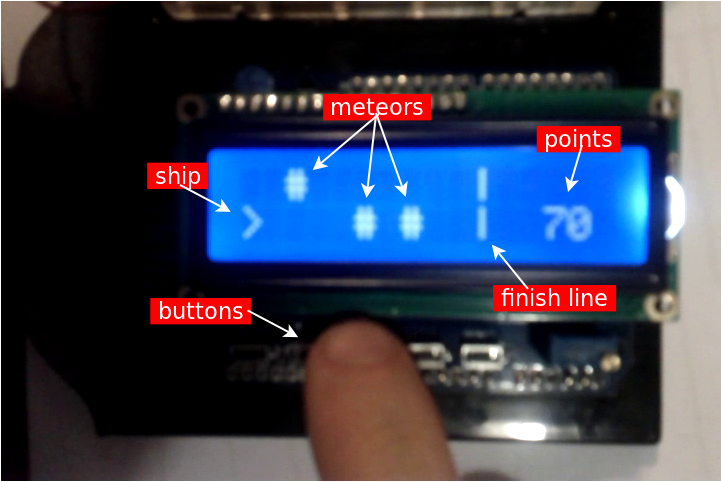
\includegraphics[scale=0.30]{ship.png}
\caption{ The ``spaceship'' game
\label{fig:ship}
}
\end{figure}

We describe the behavior of the game, along with its implementation, following 
a top-down approach.
The program is constituted of \code{CODE~1} (set game attributes), 
\code{CODE~2} (central loop), and \code{CODE~3} (game over), which are expanded 
further.
The outermost loop of the game (lines 1-61) is responsible for restarting the 
game every new phase or on ``game over'':

\newpage

{\small
\begin{verbatim}
     1:  loop do
    (2-12): // CODE 1: set game attributes
    13:
    14:     _map_generate();
    15:     _redraw(step, ship, points);
    16:     await Key;  // starting key
    17:
    18:     win =
    (19-45): // CODE 2: the central loop
    46:
    (47-60): // CODE 3: game over
    61:  end
\end{verbatim}
}

Every time the loop is executed, it resets the game attributes, such as points 
and speed (\code{CODE 1}, lines 2-12), generates a new map (line 14), redraws 
it on screen (line 15), and waits for a starting key (line 16).
Then, the program executes the main logic of the game, in the central loop, 
until the spaceship reaches the finish line or collides with a meteor 
(\code{CODE 2}, lines 19-45).
Based on the return status (line 18), the ``game over'' code (\code{CODE 3}, 
lines 47-60) may display an animation before restarting the game.

The game attributes (\code{CODE 1}) change depending on the result of the 
previous iteration of the outermost loop (held on variable \code{win}):

{\small
\begin{verbatim}
         // CODE 1: set game attributes
     2:  ship = 0;          // starts on 1st LCD row
     3:  if !win then
     4:     dt     = 500;   // game speed (500ms/step)
     5:     step   = 0;     // current step
     6:     points = 0;     // number of steps alive
     7:  else
     8:     step = 0;
     9:     if dt > 100 then
    10:        dt = dt - 50;
    11:     end
    12:  end
\end{verbatim}
}

For the first game execution and whenever the spaceship collides with a meteor, 
variable \code{win} is false, hence, the attributes are reset to their initial 
values (lines 4-6).
Otherwise, if the player reached the finish line, then the game gets faster, 
keeping the current points (lines 8-11).

The central loop of the game (\code{CODE 2}) is responsible for moving the 
spaceship as time elapses and for checking whether the spaceship reaches the 
finish line or collides with a meteor:

{\small
\begin{verbatim}
         // CODE 2: the central loop
    19:  par do
    20:     loop do
    21:        await (dt)ms;
    22:        step = step + 1;
    23:        _redraw(step, ship, points);
    24:
    25:        if _MAP[ship][step] == '#' then
    26:           return 0;  // a collision
    27:        end
    28:
    29:        if step == _FINISH then
    30:           return 1;  // finish line
    31:        end
    32:
    33:        points = points + 1;
    34:     end
    35:  with
    36:     loop do
    37:        int key = await Key;
    38:        if key == _KEY_UP then
    39:           ship = 0;
    40:        end
    41:        if key == _KEY_DOWN then
    42:           ship = 1;
    43:        end
    44:     end
    45:  end;
\end{verbatim}
}

The central loop is actually split in two loops in parallel: one that runs the 
game steps (lines 20-34), and the other that handles input from the player to 
move the spaceship (lines 36-44).
Note that we want the spaceship to move only during the game action, this is 
why we did not place the input handling in parallel with the whole application.

The game steps run periodically, depending on the current speed of the game 
(line 21).
For each loop iteration, the step is incremented and the current state is 
redrawn on screen (lines 22-23).
Then, the spaceship is checked for collision with meteors (lines 25-27), and 
also with the finish line (lines 29-31).
\CEU{} supports returning from blocks with an assignment, hence, lines 26 and 
30 escape the whole \code{par} and assign the appropriate value to variable 
\code{win} in the outermost loop (line 18), also cancelling the input handling 
activity.
The points are incremented before each iteration of the loop (line 33).

To handle input events, we wait for key presses in a loop (line 37) and change 
the spaceship position accordingly (lines 39, 42).
Note that there are no possible race conditions on variable \code{ship} (lines 
25 \emph{vs.} 39 and 42) because the two loops in the \code{par} statement 
react to different events (i.e. time and key presses).

After returning from the central loop, we run the code for the ``game over'' 
behavior, which starts an animation if the spaceship collides with a meteor:

{\small
\begin{verbatim}
         // CODE 3: game over
    47:  par/or do
    48:     await Key;
    49:  with
    50:     if !win then
    51:        loop do
    52:           await 100ms;
    53:           _lcd.setCursor(0, ship);
    54:           _lcd.write('<');
    55:           await 100ms;
    56:           _lcd.setCursor(0, ship);
    57:           _lcd.write('>');
    58:        end
    59:     end
    60:  end
\end{verbatim}
}

The animation loop (lines 51-58) continuously displays the spaceship in the two 
directions, suggesting that it has hit a meteor.
The animation is interrupted when the player presses a key (line 48), 
proceeding to the game restart.
Note the use of the \code{\_lcd} object, available in a third-party $C++$ 
library shipped with the LCD display, and used unmodified in the example.

This demo makes extensive use of global variables, relying on the
deterministic concurrency analysis guaranteed by the \CEU{} compiler.
We used a top-down approach to illustrate the hierarchical compositions of 
blocks of code.
For instance, the ``game over'' animation, which is self-contained in lines 
51-58, can be easily removed or switched for a new behavior without considering 
other parts of the program.

\newpage
\section{Related work}
\label{sec:related}

A number of previous works propose new programming languages as high-level 
alternatives to reduce code complexity in embedded 
systems~\cite{wsn.protothreads,wsn.osm,wsn.sol,arduino.occam}.
Roughly speaking, they offer adaptations to constrained platforms of classical 
programming models, such as cooperative multithreading, finite state machines, 
Esterel, and message-passing.

In cooperative multithreading, the programmer himself is responsible for 
controlling the life cycle of activities in the program (e.g. creating, 
starting, rejoining, and destroying).
With this approach, there are no possible race conditions on shared variables, 
as the points that transfer control are explicit (and, supposedly, are never 
inside critical sections).
\CEU{} goes one step further and, through parallel compositions, makes manual 
bookkeeping of activities unnecessary.

Regarding finite state machines (FSMs), they are applied in control-intensive 
algorithms, such as network protocols.
However, implementing sequential flow in FSMs is tedious, requiring to break 
programs in multiple states with a single transition connecting each of them.
Another inherent problem of FSMs is the state explosion phenomenon, which can 
be alleviated with support for parallel hierarchical FSMs~\cite{wsn.osm}.
However, adopting parallelism precludes the use of shared state, or at least 
requires a static analysis such as that of \CEU{}.

Esterel also provides an imperative reactive style with a similar set of 
parallel compositions (in which \CEU{} was based).
However, Esterel has no support for shared variables: ``if a variable is 
written in a thread, then it can be neither read nor written in any concurrent 
thread''~\cite{esterel.primer}.
We believe that shared-memory concurrency can be convenient when backed by a 
safety analysis.

Finally, message passing systems employ time independence among processes, as 
discussed in Section~\ref{sec:ceu:high}, hindering the development of highly 
synchronized applications.

None of the referred works provide a compile-time analysis that enforces 
deterministic access to shared variables and $C$ calls.
Also, some of them lack bounded execution warranties for loops 
(\cite{wsn.protothreads,wsn.sol,wsn.osm}) and fully orthogonal compositions 
(\cite{wsn.protothreads,arduino.occam}) as discussed in Section~\ref{sec:ceu}.

\section{Conclusion}
\label{sec:conclusion}

This paper promotes high-level and safe development of embedded systems through 
capabilities found in the synchronous programming language \CEU{}.
Applications can be implemented as hierarchical compositions of sequences, 
loops, assignments and parallelism.
Furthermore, support for awaiting time and events eliminates the need of 
callbacks for designing reactive systems.

The presented demos show how typical patterns in embedded systems such as 
sampling and watchdogs can be easily implemented.
They also explore parallel compositions for specifying complementary activities 
in separate.
Communication among activities can either use internal events, or safe access 
to global variables.

The synchronous execution model eliminates the need for mutual exclusion 
primitives, enabling a simpler lock-free form of concurrency.
Regarding safety, programs rely on the static analysis of \CEU{} to ensure 
deterministic behavior for concurrent access to globals and $C$ calls.
The language also guarantees bounded execution on reactions to events, which is 
an important requirement for real-time systems.

The applications are targeted at highly constrained embedded platforms, which 
fit the small memory footprint of the \CEU{} runtime (around 2Kbytes of ROM and 
50bytes of RAM).
The examples also make recurrent use of $C$ through a seamless interaction with 
globals, types, and third-party libraries from the underlying platform.

\bibliographystyle{abbrv}
\bibliography{other,my}

\end{document}
